% Abbildungen zur MQA-Extremfallanalyse (Abschnitt 5.8.2).
% Erzeugt von playground/notebooks/18_evaluation_kapitel5_final.ipynb.
% Bewusst im Anhang: Die Extremfaelle sind konstruiert und tragen keine
% verallgemeinerbare Aussage; im Fliesstext wird auf sie verwiesen.

Die folgenden vier Abbildungen entsprechen den Darstellungen aus
Abschnitt~\ref{subsec:mqa_kernstichprobe}, hier jedoch auf den zwanzig kuratierten Extremfällen statt auf
der Kernstichprobe. Sie sind nach Indikatorklasse geordnet: Konvergenz auf
Klasse~A, Überschätzung auf Klasse~B, Score-Streuung auf Klasse~C und
abschließend der Vergleich der Gesamtscores.

\begin{figure}[H]
    \centering
    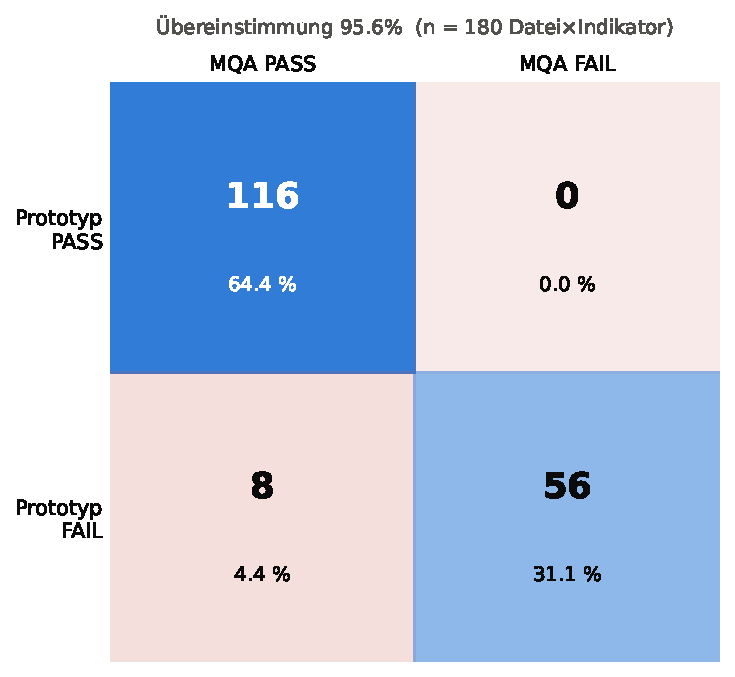
\includegraphics[width=0.55\textwidth]{images/mqa_extremfaelle_konvergenz_matrix.pdf}
    \captionsetup{justification=centering}
    \caption{Konvergenz auf Klasse-A-Indikatoren (Extremfälle, $n=180$ Datei-Indikator-Paare)}
    \label{fig:mqa_extrem_konvergenz}
\end{figure}

\begin{figure}[H]
    \centering
    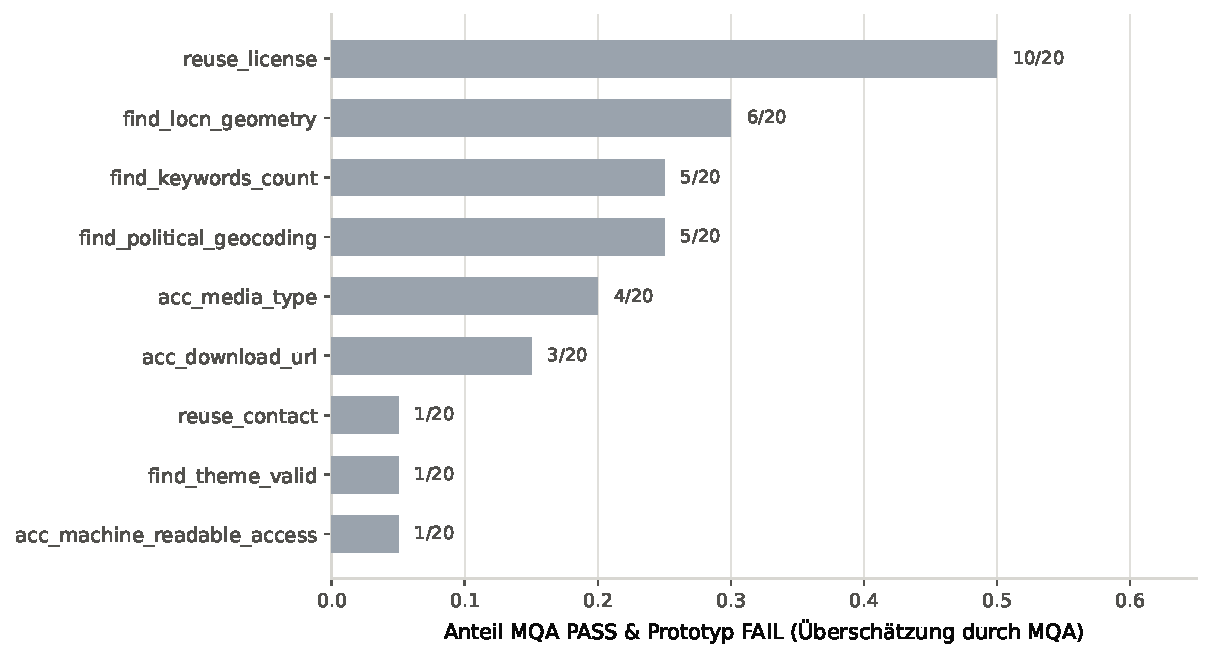
\includegraphics[width=0.85\textwidth]{images/mqa_extremfaelle_ueberschaetzung.pdf}
    \captionsetup{justification=centering}
    \caption{Überschätzungsrate je Klasse-B-Indikator: Anteil MQA PASS \& Prototyp FAIL (Extremfälle)}
    \label{fig:mqa_extrem_ueberschaetzung}
\end{figure}

\begin{figure}[H]
    \centering
    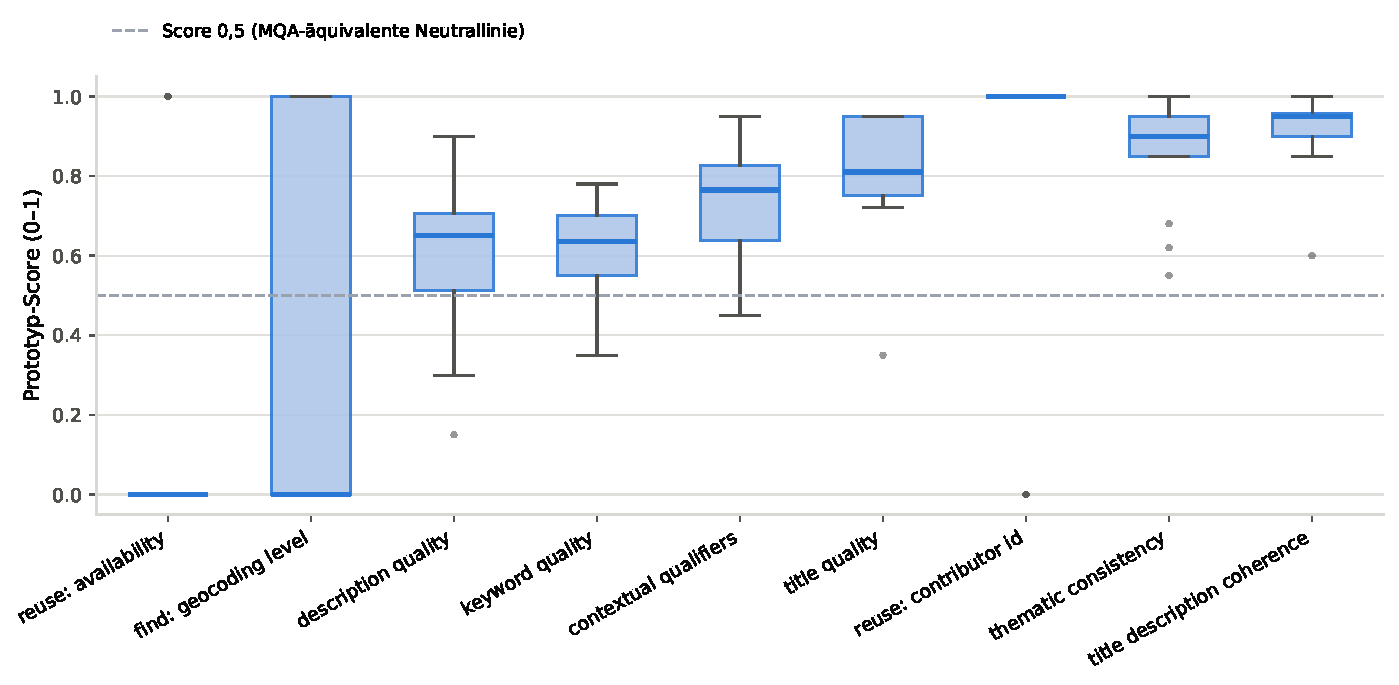
\includegraphics[width=\textwidth]{images/mqa_extremfaelle_blindheit_boxplot.pdf}
    \captionsetup{justification=centering}
    \caption{Prototyp-Score-Verteilung auf Klasse-C-Indikatoren, für die die MQA keine Metrik besitzt (Extremfälle)}
    \label{fig:mqa_extrem_blindheit}
\end{figure}

\begin{figure}[H]
    \centering
    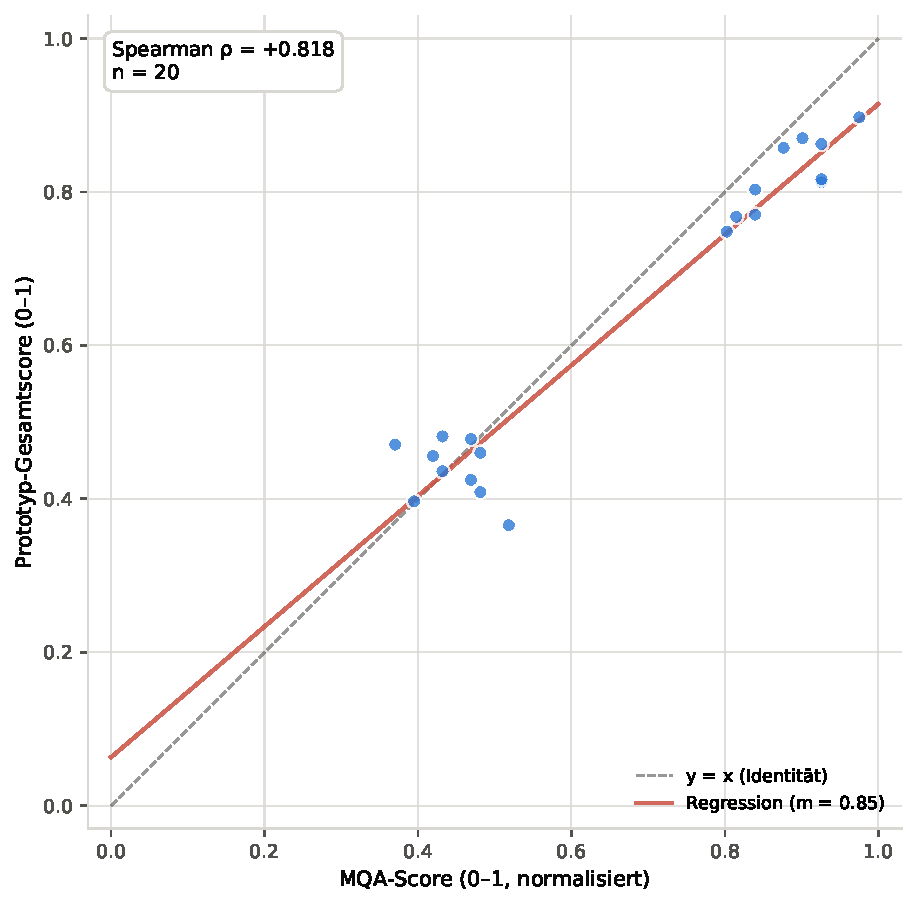
\includegraphics[width=0.62\textwidth]{images/mqa_extremfaelle_scatter_gesamt.pdf}
    \captionsetup{justification=centering}
    \caption{Gesamtscore Prototyp vs. MQA (Extremfälle, $n=20$)}
    \label{fig:mqa_extrem_scatter}
\end{figure}

\pagebreak